% Proposed revision of "Language Extension: Fuel Inference" section
% This version covers both fuel inference AND session type tracking
% 
% To compile standalone:
%   pdflatex fuel_session_section_proposal.tex
%
% To include in main paper, copy the content between BEGIN/END markers

\documentclass[11pt]{article}
\usepackage[utf8]{inputenc}
\usepackage{amsmath,amssymb}
\usepackage{minted}
\usepackage{tikz}
\usetikzlibrary{arrows.meta, positioning, shapes.geometric, decorations.pathreplacing, calc}
\usepackage{xcolor}
\usepackage{hyperref}

% Match paper's Coq inline style
\newcommand{\coqin}[1]{\texttt{#1}}
\newcommand{\coq}{\textsc{Coq}}

\begin{document}

\title{Proposed Section: Language Extension with Fuel and Session Type Inference}
\author{Draft for ITP 2026 Paper}
\date{January 25, 2026}
\maketitle

% ============================================================================
% BEGIN PROPOSED SECTION
% ============================================================================

\section{Language Extension: Fuel and Session Type Inference}
\label{sec:fuel-session-inference}

The protocol description language of Weng et al.\ is defined as an inductive
type in \coq{} with an explicit fuel parameter that serves as a termination
measure. In their formulation, the fuel value must be chosen manually---a
tedious and error-prone process. Miscounting leads either to incomplete
execution (fuel exhausted too early) or to wasted proof obligations
(fuel larger than needed).

We address this with a \emph{two-layer architecture}. The \textbf{session
layer} defines a type \coqin{sproc} indexed by both fuel \emph{and} session
types; \coq{}'s unification mechanism infers both automatically from the
program structure. The \textbf{core layer} provides an \emph{unindexed}
\coqin{proc} type for interpretation and relational semantics proofs.
An erasure function bridges the layers, stripping both indices. Crucially,
before erasure we \emph{extract} the inferred fuel to pass to the
interpreter---eliminating manual fuel specification entirely.

Building on this foundation, we add \emph{binary session types}~\cite{honda1998}
to the session layer, enabling static verification that communicating parties
have compatible (dual) communication patterns. Both fuel and session indices
are inferred simultaneously, preserving the paper-like surface syntax.

\subsection{Architecture Overview}

Figure~\ref{fig:fuel-session-architecture} illustrates the layered architecture.
The \textbf{core layer} provides an \emph{unindexed} \coqin{proc} type and
interpreter---simplified from Weng et al.\ by removing type indices entirely.
The \textbf{session layer} defines a session-indexed \coqin{sproc} type that
tracks both fuel and per-party session environments; both indices are
automatically inferred by \coq{}'s unification. The \textbf{surface layer}
uses \coq{} custom entries to provide paper-like syntax that hides the type
machinery. An \textbf{erasure function} strips both indices, bridging
session-typed programs back to the unindexed interpreter. Crucially, the
inferred fuel is \emph{extracted} before erasure, eliminating the need
to manually specify interpreter bounds.

\begin{figure}[htbp]
  \centering
  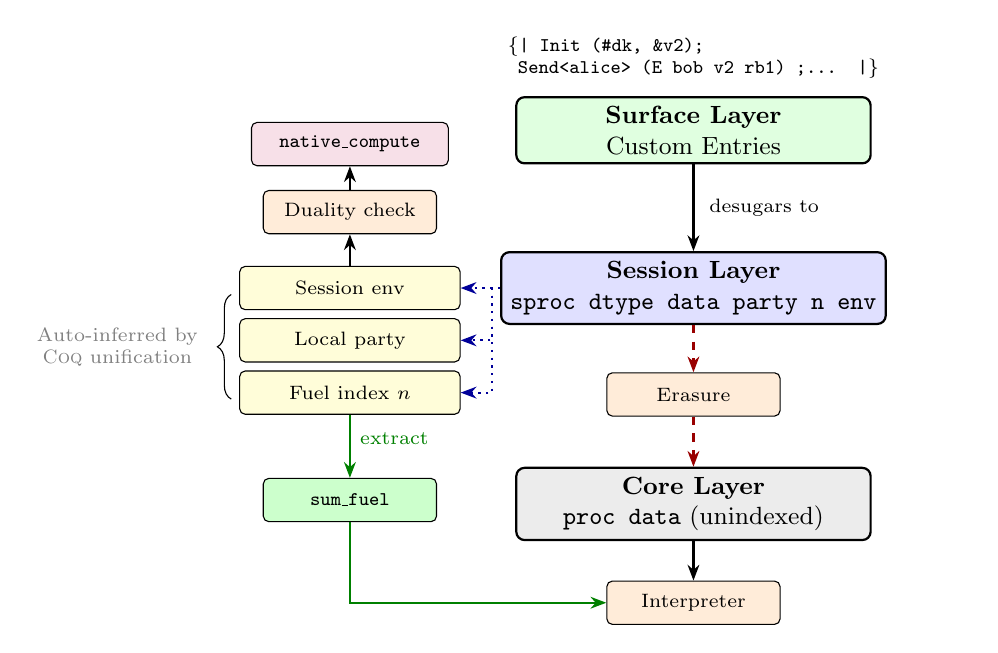
\begin{tikzpicture}[
    node distance=0.7cm and 1.2cm,
    every node/.style={font=\small},
    % Box styles
    corebox/.style={
      rectangle, draw, thick, rounded corners=3pt,
      minimum width=4.5cm, minimum height=0.8cm,
      fill=gray!15
    },
    sessionbox/.style={
      rectangle, draw, thick, rounded corners=3pt,
      minimum width=4.5cm, minimum height=0.8cm,
      fill=blue!12
    },
    surfacebox/.style={
      rectangle, draw, thick, rounded corners=3pt,
      minimum width=4.5cm, minimum height=0.8cm,
      fill=green!12
    },
    notebox/.style={
      rectangle, draw=none, 
      font=\scriptsize, align=left,
      fill=white, inner sep=2pt
    },
    indexbox/.style={
      rectangle, draw, rounded corners=2pt,
      minimum width=2.8cm, minimum height=0.55cm,
      fill=yellow!15, font=\scriptsize
    },
    opbox/.style={
      rectangle, draw, rounded corners=2pt,
      minimum width=2.2cm, minimum height=0.55cm,
      fill=orange!15, font=\scriptsize
    },
    proofbox/.style={
      rectangle, draw, rounded corners=2pt,
      minimum width=2.5cm, minimum height=0.55cm,
      fill=purple!12, font=\scriptsize
    },
    fuelbox/.style={
      rectangle, draw, rounded corners=2pt,
      minimum width=2.2cm, minimum height=0.55cm,
      fill=green!20, font=\scriptsize
    },
    % Arrow styles
    arr/.style={-{Stealth[length=2mm]}, thick},
    erasearr/.style={-{Stealth[length=2mm]}, thick, dashed, color=red!60!black},
    inferarr/.style={-{Stealth[length=2mm]}, dotted, thick, color=blue!60!black},
    fuelarr/.style={-{Stealth[length=2mm]}, thick, color=green!50!black}
  ]
  
  % ============ Core Layer (Bottom) ============
  \node[corebox, align=center] (core)
    {\textbf{Core Layer}\\ \coqin{proc data} (unindexed)};
  \node[opbox, below=0.5cm of core] (interp) {Interpreter};
  
  % ============ Session Layer (Middle) ============
  \node[sessionbox, above=1.8cm of core, align=center] (session) 
    {\textbf{Session Layer}\\ \coqin{sproc dtype data party n env}};
  \node[indexbox, left=0.5cm of session] (envidx) {Session env};
  \node[indexbox, below=0.1cm of envidx] (partyidx) {Local party};
  \node[indexbox, below=0.1cm of partyidx] (fuelidx) {Fuel index $n$};
  
  % ============ Session Operations ============
  \node[opbox, below=0.6cm of session] (erase) {Erasure};
  \node[fuelbox, below=0.8cm of fuelidx] (sumfuel) {\coqin{sum\_fuel}};
  \node[opbox, above=0.4cm of envidx] (dual) {Duality check};
  \node[proofbox, above=0.3cm of dual] (dualproof) 
    {\coqin{native\_compute}};

  % ============ Surface Layer (Top) ============
  \node[surfacebox, above=1.1cm of session, align=center] (surface) 
    {\textbf{Surface Layer}\\ Custom Entries};
  
  % ============ Example syntax ============
  \node[above=0.1cm of surface, font=\ttfamily\scriptsize, align=left] (syntax)
    {\{| Init (\#dk, \&v2);\\~Send<alice> (E bob v2 rb1) ;... |\}};
  
  % ============ Arrows ============
  % Surface to Session
  \draw[arr] (surface) -- (session) 
    node[midway, right, font=\scriptsize, xshift=2pt] {desugars to};
  
  % Session indices (inferred)
  \draw[inferarr] (session.west) |- ++(-0.1,-0.0) |- (partyidx.east)
    node[midway, above, font=\scriptsize] {};
  \draw[inferarr] (session.west) -- (envidx.east)
    node[midway, above, font=\scriptsize] {};
  \draw[inferarr] (session.west) |- ++(-0.1,-0.0) |- (fuelidx.east)
    node[pos=0.5, left, font=\scriptsize] {};
  
  % Session operations
  \draw[arr] (envidx) -- (dual);
  \draw[arr] (dual) -- (dualproof);
  \draw[erasearr] (session) -- (erase);
  \draw[erasearr] (erase.south) -- (core.north)
    node[pos=0.5, right, font=\scriptsize, color=red!60!black] {};
  
  % Fuel extraction and passing
  \draw[fuelarr] (fuelidx.south) -- ++(0,-0.3) -| (sumfuel.north)
    node[pos=0.1, right, font=\scriptsize, color=green!50!black] {extract};
  \draw[fuelarr] (sumfuel.south) |- (interp.west)
    node[pos=0.2, right, font=\scriptsize, color=green!50!black] {};
  
  % Core to interpreter
  \draw[arr] (core) -- (interp);
  
  % ============ Layer labels ============
  \node[right=1.0cm of core, font=\scriptsize, text=gray, align=left] (l1)
    {};
  \node[left=1.0cm of session, font=\scriptsize, text=gray, align=left] (l2)
    {};
  \node[right=0.2cm of surface, font=\scriptsize, text=gray, align=left] (l3)
    {};
  
  % ============ Brace for indices ============
  \draw[decorate, decoration={brace, amplitude=5pt, mirror}]
    ([yshift=0.2cm, xshift=-0.1cm]envidx.south west) -- ([yshift=0.2cm, xshift=-0.1cm]fuelidx.south west)
    node[align=center, midway, left=0.3cm, font=\scriptsize, text=gray] 
    {Auto-inferred by\\ \coq{} unification};
    
  \end{tikzpicture}
  \caption{Two-layer architecture for fuel and session type inference.
    The \textbf{core layer} provides \emph{unindexed} processes and the interpreter,
    simplifying relational semantics proofs.
    The \textbf{session layer} adds three indices: the \emph{local party},
    the \emph{fuel} $n$, and the \emph{session environment}---all inferred by
    \coq{}'s unification.
    The \textbf{surface layer} uses custom entries for paper-like syntax.
    Dotted blue arrows show automatic inference; dashed red arrows show erasure
    that strips \emph{both} indices for interpretation; green arrows show
    automatic fuel extraction via \coqin{sum\_fuel}.}
  \label{fig:fuel-session-architecture}
\end{figure}

\subsection{Core Layer: Unindexed Processes}

The core process type is \emph{unindexed}---it carries no type-level
information about fuel or session types:

\begin{minted}[fontsize=\small,escapeinside=77]{coq}
Inductive proc : Type :=
| Init   : data 7$\to$7 proc 7$\to$7 proc
| Send   : 7$\mathbb{N}$7 7$\to$7 data 7$\to$7 proc 7$\to$7 proc
| Recv   : 7$\mathbb{N}$7 7$\to$7 (data 7$\to$7 proc) 7$\to$7 proc
| Ret    : data 7$\to$7 proc
| Finish : proc
| Fail   : proc.
\end{minted}

This simplification from Weng et al.'s fuel-indexed version has two benefits:
(1)~the interpreter and step function become simpler, with no dependent
pattern matching on indices; and (2)~relational semantics proofs (e.g.,
soundness of the step function) avoid the complexity of heterogeneous
fuel indices in tuples. The session layer handles type-level tracking;
the core layer focuses solely on execution.

\subsection{Surface Syntax via Custom Entries}

Writing raw constructors like \coqin{SInit}, \coqin{SSend}, \coqin{SRecv}
is verbose and obscures the protocol logic. We use \coq{}'s custom entry
mechanism to provide paper-like syntax. The delimiters \coqin{\{|} and
\coqin{|\}} enter and exit the custom entry; within it, we define notations:

\begin{minted}[fontsize=\small]{coq}
Notation "'Init' x ; P" := (SInit x P).
Notation "'Send<' p '>' x ; P" := (SSend p DT_Enc x P).
Notation "'Recv_dec<' p '>' dk 'fun' x '=>' P" := (SRecv p DT_Enc ...).
Notation "'Finish'" := SFinish.
\end{minted}

\noindent
With these notations, a protocol reads like pseudocode:

\begin{minted}[fontsize=\small]{coq}
Definition pbob (dk : pkey)(v2 : msg)(rb1 rb2 : rand)
    : @sproc dsdp_dtype data bob_idx _ _ :=
  {| Init (#dk, &v2) ;
     Send<alice_idx> (E bob v2 rb1) ;
     Recv_dec<alice_idx> dk fun d2 =>
     Recv_enc<alice_idx> fun a3 =>
     Send<charlie_idx> (a3 *h (E charlie d2 rb2)) ;
     Finish |}.
\end{minted}

\noindent
The underscores in the type signature are placeholders for the fuel and
session environment indices, which \coq{} infers automatically.

\subsection{Type-Indexed Inference via Unification}

The key to automatic inference is \emph{type indexing}: each constructor's
return type explicitly computes the index from its arguments. When a user
writes \coqin{proc data \_}, the underscore is a \emph{unification variable}
that \coq{}'s type checker must solve.

\paragraph{The Backwards Building Insight.}
A subtlety arises with session types: we write programs \emph{forwards}
(from start to end), but session types accumulate \emph{backwards}
(from end to start). For example:
\[
\begin{array}{lcl}
\textbf{Code (forwards)} & & \textbf{Session type (backwards)} \\[2pt]
\coqin{Send<bob> enc1} & & \mathsf{STSend~DT\_Enc} \\
\coqin{Send<bob> enc2} & \longrightarrow & \quad(\mathsf{STSend~DT\_Enc} \\
\coqin{Finish} & & \quad\quad\mathsf{STEnd}))
\end{array}
\]
The solution exploits how \coq{} type-checks inductive terms: it processes
the \emph{continuation first}, then the \emph{wrapper}. Consider the
\coqin{SSend} constructor's type:
\begin{minted}[fontsize=\small,escapeinside=77]{coq}
| SSend : 7$\forall$7 n env dst dt, data 7$\to$7 sproc party n env 7$\to$7
            sproc party n.+1 (senv_send env dst dt)
\end{minted}
The continuation argument has type \coqin{sproc party n env}---its session
environment \coqin{env} is determined \emph{before} the wrapper is checked.
The wrapper's return type then \emph{prepends} via \coqin{senv\_send}:
\begin{minted}[fontsize=\small]{coq}
Definition senv_send env dst dt :=
  fun p => if p == dst then STSend dt (env p) else env p.
\end{minted}
Thus, when \coq{} checks \coqin{SSend dst dt d (SSend dst dt d' SFinish)}:
\begin{enumerate}
  \item It first checks \coqin{SFinish}, which has \coqin{env = senv\_end}
  \item The inner \coqin{SSend} prepends, yielding \coqin{senv\_send senv\_end dst dt}
  \item The outer \coqin{SSend} prepends again, yielding the final environment
\end{enumerate}
Because \coq{} processes inside-out, session types naturally accumulate
in the correct (backwards) order. The base case \coqin{SFinish} anchors the
environment at \coqin{senv\_end}, and each wrapper prepends its contribution.

\paragraph{Unification in Action.}
Consider building a process bottom-up:

\begin{enumerate}
  \item \coqin{Finish} has type \coqin{proc 1} (base case: fuel = 1)
  \item \coqin{Send dst d Finish} has type \coqin{proc (1+1) = proc 2}
  \item \coqin{Init x (Send dst d Finish)} has type \coqin{proc (2+1) = proc 3}
\end{enumerate}

\noindent
At each step, the constructor's type signature \emph{computes} the resulting
index. \coq{}'s unification engine propagates these constraints, solving for
the underscore without user intervention.

We extend this principle to session types. The \coqin{SSend} constructor's
return type includes \coqin{senv\_send env dst dt}, which \emph{prepends}
$\mathsf{!}dt$ to the session environment. Similarly, \coqin{SRecv} prepends
$\mathsf{?}dt$. The session environment accumulates as the term is built,
and \coq{} unifies it automatically.

\paragraph{Concrete Example.}
Consider a simple protocol where Bob (party index \coqin{bob\_idx = 1})
initializes a key, sends an encrypted value to Alice (party index
\coqin{alice\_idx = 0}), then finishes:

\begin{minted}[fontsize=\small]{coq}
Definition pbob : @sproc dsdp_dtype data bob_idx _ _ :=
  {| Init #dk ;
     Send<alice_idx> (E bob v2 rb1) ;
     Finish |}.
\end{minted}

\noindent
The two underscores are unification variables. The custom entry desugars to
raw constructors, which \coq{} then type-checks bottom-up:

\begin{itemize}
  \item \textbf{Fuel} (first underscore): Building bottom-up:
    \begin{itemize}
      \item \coqin{Finish} $\mapsto$ \coqin{SFinish} has fuel 1
      \item \coqin{Send<alice\_idx> ...} $\mapsto$ \coqin{SSend alice\_idx ...} has fuel $1+1 = 2$
      \item \coqin{Init \#dk} $\mapsto$ \coqin{SInit (k dk) ...} has fuel $2+1 = 3$
    \end{itemize}
    Thus the first underscore becomes \textbf{3}.
    
  \item \textbf{Session environment} (second underscore): Building bottom-up:
    \begin{itemize}
      \item \coqin{SFinish} has environment $\mathsf{senv\_end} = \lambda p.\, \mathsf{STEnd}$
      \item \coqin{SSend alice\_idx DT\_Enc ...} prepends $\mathsf{!DT\_Enc}$ to Alice's session:
        \[
          \lambda p.\, \mathsf{if}~p = \mathit{alice\_idx}~\mathsf{then}~\mathsf{STSend}~\mathsf{DT\_Enc}~\mathsf{STEnd}~\mathsf{else}~\mathsf{STEnd}
        \]
      \item \coqin{SInit ...} does not affect the session environment
    \end{itemize}
    Thus the second underscore becomes
    $\lambda p.\, \mathsf{if}~p = 0~\mathsf{then}~\mathsf{!DT\_Enc.end}~\mathsf{else}~\mathsf{end}$.
\end{itemize}

\noindent
In other words, \coq{} infers that Bob's process requires 3 steps of fuel and
has session type $\mathsf{!DT\_Enc.end}$ with Alice. For duality to hold,
Alice must have session type $\mathsf{?DT\_Enc.end}$ with Bob---exactly
the dual.

Figure~\ref{fig:unification-flow} illustrates the inference workflow:
the developer writes a definition with underscores, \coq{}'s unification
solves for both fuel and session environment, and duality verification
reduces to a computational check.

\begin{figure}[htbp]
  \centering
  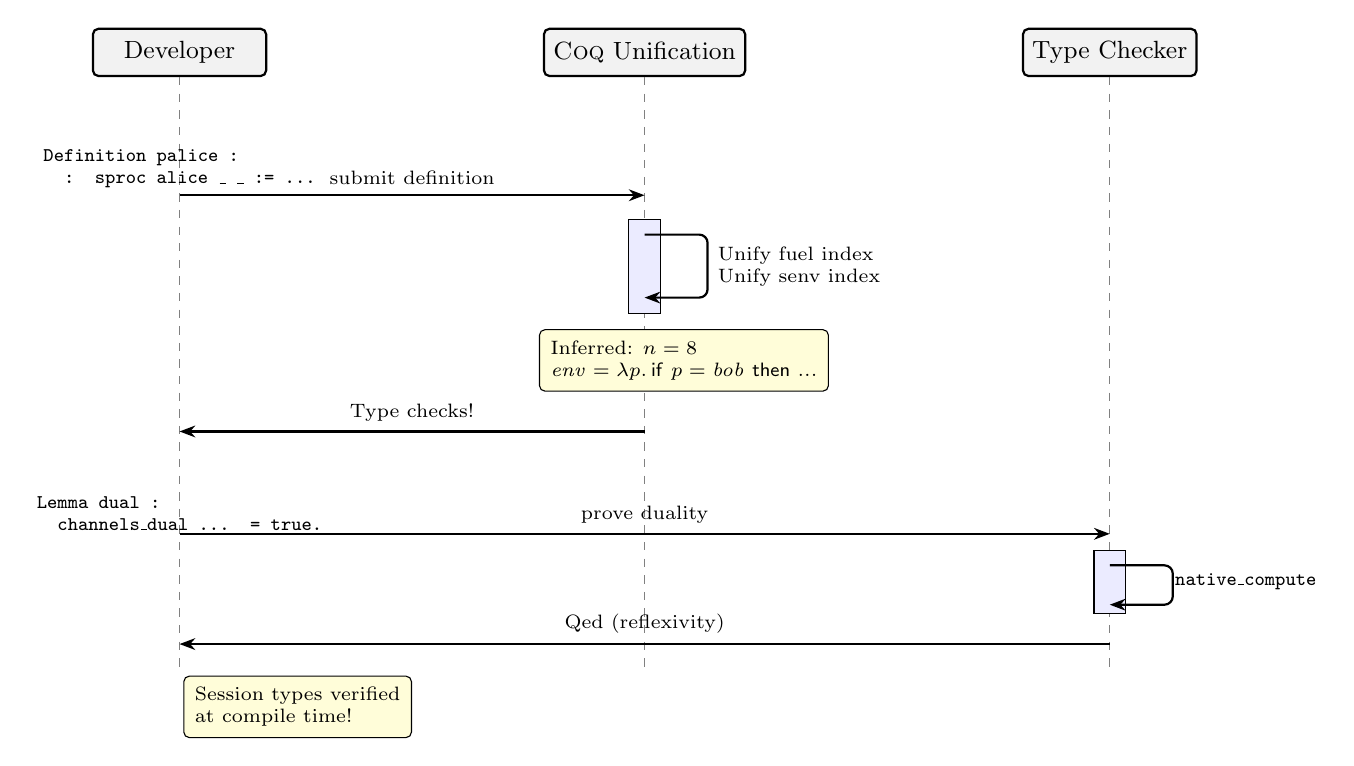
\begin{tikzpicture}[
    node distance=0.8cm,
    every node/.style={font=\small},
    % Actor boxes
    actorbox/.style={
      rectangle, draw, thick, rounded corners=2pt,
      minimum width=2.2cm, minimum height=0.6cm,
      fill=gray!10
    },
    % Lifeline
    lifeline/.style={dashed, gray},
    % Message arrow
    msgarr/.style={-{Stealth[length=2mm]}, thick},
    selfarr/.style={-{Stealth[length=2mm]}, thick, rounded corners=3pt},
    % Note box
    notebox/.style={
      rectangle, draw, rounded corners=2pt,
      fill=yellow!15, font=\scriptsize, align=left,
      inner sep=4pt
    },
    % Action box
    actionbox/.style={
      rectangle, draw, fill=blue!8,
      minimum width=0.4cm, minimum height=1.2cm
    }
  ]
  
  % ============ Actors ============
  \node[actorbox] (dev) {Developer};
  \node[actorbox, right=3.5cm of dev] (coq) {\coq{} Unification};
  \node[actorbox, right=3.5cm of coq] (check) {Type Checker};
  
  % ============ Lifelines ============
  \draw[lifeline] (dev.south) -- ++(0,-7.5);
  \draw[lifeline] (coq.south) -- ++(0,-7.5);
  \draw[lifeline] (check.south) -- ++(0,-7.5);
  
  % ============ Step 1: Definition ============
  \node[below=0.8cm of dev, font=\ttfamily\scriptsize, align=left] (def) 
    {Definition palice :\\~~: sproc alice \_ \_ := ...};
  \draw[msgarr] ([yshift=-1.5cm]dev.south) -- ([yshift=-1.5cm]coq.south)
    node[midway, above, font=\scriptsize] {submit definition};
  
  % ============ Step 2: Unification ============
  \node[actionbox, below=1.8cm of coq] (unifyact) {};
  \draw[selfarr] ([yshift=-2.0cm]coq.south) -- ++(0.8,0) -- ++(0,-0.8) -- ++(-0.8,0);
  \node[right=0.6cm of unifyact, font=\scriptsize, align=left] (unifylbl)
    {Unify fuel index\\Unify senv index};
  
  % ============ Note: inference result ============
  \node[notebox, below=3.2cm of coq, xshift=0.5cm] (infernote)
    {Inferred: $n = 8$\\$\mathit{env} = \lambda p.\, \mathsf{if}~p = \mathit{bob}~\mathsf{then}~...$};
  
  % ============ Step 3: Type checks ============
  \draw[msgarr] ([yshift=-4.5cm]coq.south) -- ([yshift=-4.5cm]dev.south)
    node[midway, above, font=\scriptsize] {Type checks!};
  
  % ============ Step 4: Duality proof ============
  \node[below=5.2cm of dev, font=\ttfamily\scriptsize, align=left] (proof)
    {Lemma dual :\\~~channels\_dual ... = true.};
  \draw[msgarr] ([yshift=-5.8cm]dev.south) -- ([yshift=-5.8cm]check.south)
    node[midway, above, font=\scriptsize] {prove duality};
  
  % ============ Step 5: native_compute ============
  \node[actionbox, below=6.0cm of check, minimum height=0.8cm] (compact) {};
  \draw[selfarr] ([yshift=-6.2cm]check.south) -- ++(0.8,0) -- ++(0,-0.5) -- ++(-0.8,0);
  \node[right=0.5cm of compact, font=\scriptsize] (complbl) {\coqin{native\_compute}};
  
  % ============ Step 6: Qed ============
  \draw[msgarr] ([yshift=-7.2cm]check.south) -- ([yshift=-7.2cm]dev.south)
    node[midway, above, font=\scriptsize] {Qed (reflexivity)};
  
  % ============ Final note ============
  \node[notebox, below=7.6cm of dev, xshift=1.5cm] (finalnote)
    {Session types verified\\at compile time!};
  
  \end{tikzpicture}
  \caption{Inference workflow. The developer writes a definition with
    underscores for fuel and session environment. \coq{}'s unification
    engine solves these constraints by propagating type indices through
    the term structure. Duality verification then reduces to a boolean
    equality check via \coqin{native\_compute}.}
  \label{fig:unification-flow}
\end{figure}

\subsection{Session Layer: Session-Indexed Processes}

We extend the type index to track communication patterns. In a multi-party
protocol, each party has its own \emph{local view} of the communication:
what party~$A$ sees as ``send to $B$'' is what party~$B$ sees as ``receive
from $A$.'' We capture this by indexing each process by \emph{which party
executes it} and by a \emph{session environment} that maps
each remote party to the session type for communication with that party.

A \emph{session type} describes the local party's view of communication
with a specific remote party:

\begin{minted}[fontsize=\small,escapeinside=77]{coq}
Inductive stype : Type :=
| STSend : dtype 7$\to$7 stype 7$\to$7 stype   (* !d.S - send data of kind d *)
| STRecv : dtype 7$\to$7 stype 7$\to$7 stype   (* ?d.S - receive data of kind d *)
| STEnd  : stype.                    (* session finished *)
\end{minted}

The parameter \coqin{dtype} is a user-defined type classifying data kinds
(e.g., \coqin{DT\_Enc} for encrypted values). A \emph{session environment}
maps each party identifier to the session type for communication with that
party:

\begin{minted}[fontsize=\small]{coq}
Definition senv : Type := nat -> stype.
\end{minted}

The session-indexed process type \coqin{sproc} extends \coqin{proc} with
three additional indices: the \emph{local party} whose
perspective this process represents, the fuel bound ($n$), and the
session environment ($\mathit{env}$) mapping remote parties to session types:

\begin{minted}[fontsize=\small,escapeinside=77]{coq}
Inductive sproc (party : nat) : nat 7$\to$7 senv 7$\to$7 Type :=
| SFinish : sproc party 1 senv_end
| SRet    : data 7$\to$7 sproc party 2 senv_end
| SInit   : 7$\forall$7 n env, data 7$\to$7 sproc party n env 7$\to$7 sproc party (n.+1) env
| SSend   : 7$\forall$7 n env dst dt, data 7$\to$7 sproc party n env 7$\to$7
              sproc party (n.+1) (senv_send env dst dt)
| SRecv   : 7$\forall$7 n env src dt, (data 7$\to$7 sproc party n env) 7$\to$7
              sproc party (n.+1) (senv_recv env src dt)
| SFail   : 7$\forall$7 n env, sproc party n env.
\end{minted}

The key insight is that each \coqin{SSend} and \coqin{SRecv} constructor
\emph{prepends} to the session environment: \coqin{senv\_send env dst dt}
adds $\mathsf{!}dt$ to the session with party $\mathit{dst}$.
Because session types build backwards (from end to start) while programs
are written forwards, this prepending correctly accumulates the session type.

\subsection{Duality Verification}

Two parties have \emph{dual} session types if every send by one party
corresponds to a receive by the other:

\begin{minted}[fontsize=\small]{coq}
Fixpoint dual (s : stype) : stype :=
  match s with
  | STSend d k => STRecv d (dual k)
  | STRecv d k => STSend d (dual k)
  | STEnd => STEnd
  end.

Definition channels_dual (ap1 ap2 : aproc) : bool :=
  are_dual (aproc_stype ap1 (aproc_party ap2))
           (aproc_stype ap2 (aproc_party ap1)).
\end{minted}

Because session environments are computed structurally, duality checks
reduce to boolean equality tests that \coqin{native\_compute} evaluates
in milliseconds:

\begin{minted}[fontsize=\small]{coq}
Lemma alice_bob_dual : channels_dual aproc_alice aproc_bob = true.
Proof. by native_compute. Qed.
\end{minted}

\subsection{Erasure to Core Interpreter}

Session-typed programs must ultimately execute on the core interpreter.
The \coqin{erase} function strips \emph{both} the session environment
\emph{and} the fuel index, producing an unindexed \coqin{proc}:

\begin{minted}[fontsize=\small,escapeinside=77]{coq}
Fixpoint erase {party n env} (p : sproc party n env) : proc :=
  match p with
  | SFinish => Finish
  | SRet d => Ret d
  | SInit d k => Init d (erase k)
  | SSend dst _ d k => Send dst d (erase k)
  | SRecv src _ f => Recv src (fun d => erase (f d))
  | SFail => Fail
  end.
\end{minted}

\paragraph{Automatic Fuel Extraction.}
Before erasure, we extract the inferred fuel index to pass to the interpreter.
For a list of session-typed processes, \coqin{sum\_fuel} computes the total:

\begin{minted}[fontsize=\small]{coq}
Definition sum_fuel (ps : seq aproc) : nat :=
  foldr (fun p acc => aproc_fuel p + acc) 0 ps.

Definition run_sprocs (aps : seq aproc) :=
  run_interp [> aps] (erase_aprocs aps).
\end{minted}

The notation \coqin{[> aps]} expands to \coqin{sum\_fuel aps}. This eliminates
manual fuel specification---the interpreter runs with exactly the fuel that
\coq{} inferred from the program structure.

The session layer thus acts as a \emph{refinement} of the core layer: it adds
static guarantees (session type duality) and automatic fuel computation
without changing runtime behavior.

\subsection{Termination and Well-Typedness by Reflexivity}

Both termination (from fuel inference) and protocol compatibility (from
session type inference) can be verified by \coqin{reflexivity}:

\begin{minted}[fontsize=\small]{coq}
(* Pack session-typed processes with automatic fuel extraction *)
Definition procs := [aprocs palice; pbob; pcharlie].

(* Termination: inferred fuel is sufficient *)
Lemma dsdp_terminates :
  all_final (run_sprocs procs).1.
Proof. reflexivity. Qed.

(* Duality: all channel pairs are compatible *)
Lemma alice_bob_dual : channels_dual aproc_alice aproc_bob = true.
Proof. by native_compute. Qed.

Lemma alice_charlie_dual : channels_dual aproc_alice aproc_charlie = true.
Proof. by native_compute. Qed.

Lemma bob_charlie_dual : channels_dual aproc_bob aproc_charlie = true.
Proof. by native_compute. Qed.
\end{minted}

The \coqin{reflexivity} and \coqin{native\_compute} proofs succeed because
\coq{} evaluates the computed indices and checks structural equality.
The \coqin{run\_sprocs} function automatically extracts and sums the inferred
fuel indices via \coqin{sum\_fuel}, then erases the session types for
interpretation. This closes the gap between the inferred bounds and actual
execution, eliminating the guesswork that plagued manual selection while
adding static communication safety guarantees.

% ============================================================================
% END PROPOSED SECTION
% ============================================================================

\section*{Notes for Integration}

\begin{enumerate}
  \item The TikZ diagram uses the same style conventions as
        Figure~\ref{fig:phe-hierarchy} in the original paper (box styles,
        arrow styles, color scheme).
  
  \item The section assumes the reader is familiar with binary session types
        from Honda et al.\ (1998). A brief citation suffices; detailed
        background is not needed for the ITP audience.
  
  \item The code examples use the actual notation from
        \texttt{dsdp\_program\_alt\_syntax.v} after the session type migration.
  
  \item \textbf{Two-layer design}: The core \coqin{proc} type is now
        \emph{unindexed} (no fuel parameter), while the session layer
        \coqin{sproc} tracks both fuel and session types. This separation:
        \begin{itemize}
          \item Simplifies relational semantics proofs (no heterogeneous
                fuel indices in tuples)
          \item Enables automatic fuel extraction via \coqin{sum\_fuel}
          \item Keeps erasure simple (just strip indices)
        \end{itemize}
  
  \item The erasure function demonstrates that session types are a
        \emph{refinement}---they add static guarantees without changing
        runtime semantics, which is important for soundness arguments.
  
  \item \textbf{Automatic fuel}: The \coqin{run\_sprocs} helper eliminates
        manual fuel specification entirely. Users never write explicit fuel
        bounds; \coq{} infers them and \coqin{sum\_fuel} extracts them.
\end{enumerate}

\bibliographystyle{plain}
\begin{thebibliography}{9}
\bibitem{honda1998}
Kohei Honda, Vasco T.\ Vasconcelos, and Makoto Kubo.
\newblock Language primitives and type discipline for structured
  communication-based programming.
\newblock In \emph{ESOP 1998}, LNCS 1381, pp.\ 122--138. Springer, 1998.
\end{thebibliography}

\end{document}
